\chapter{Proposition de modélisation}

\section{Le MCD}

\begin{figure}[!h]
\begin{center}
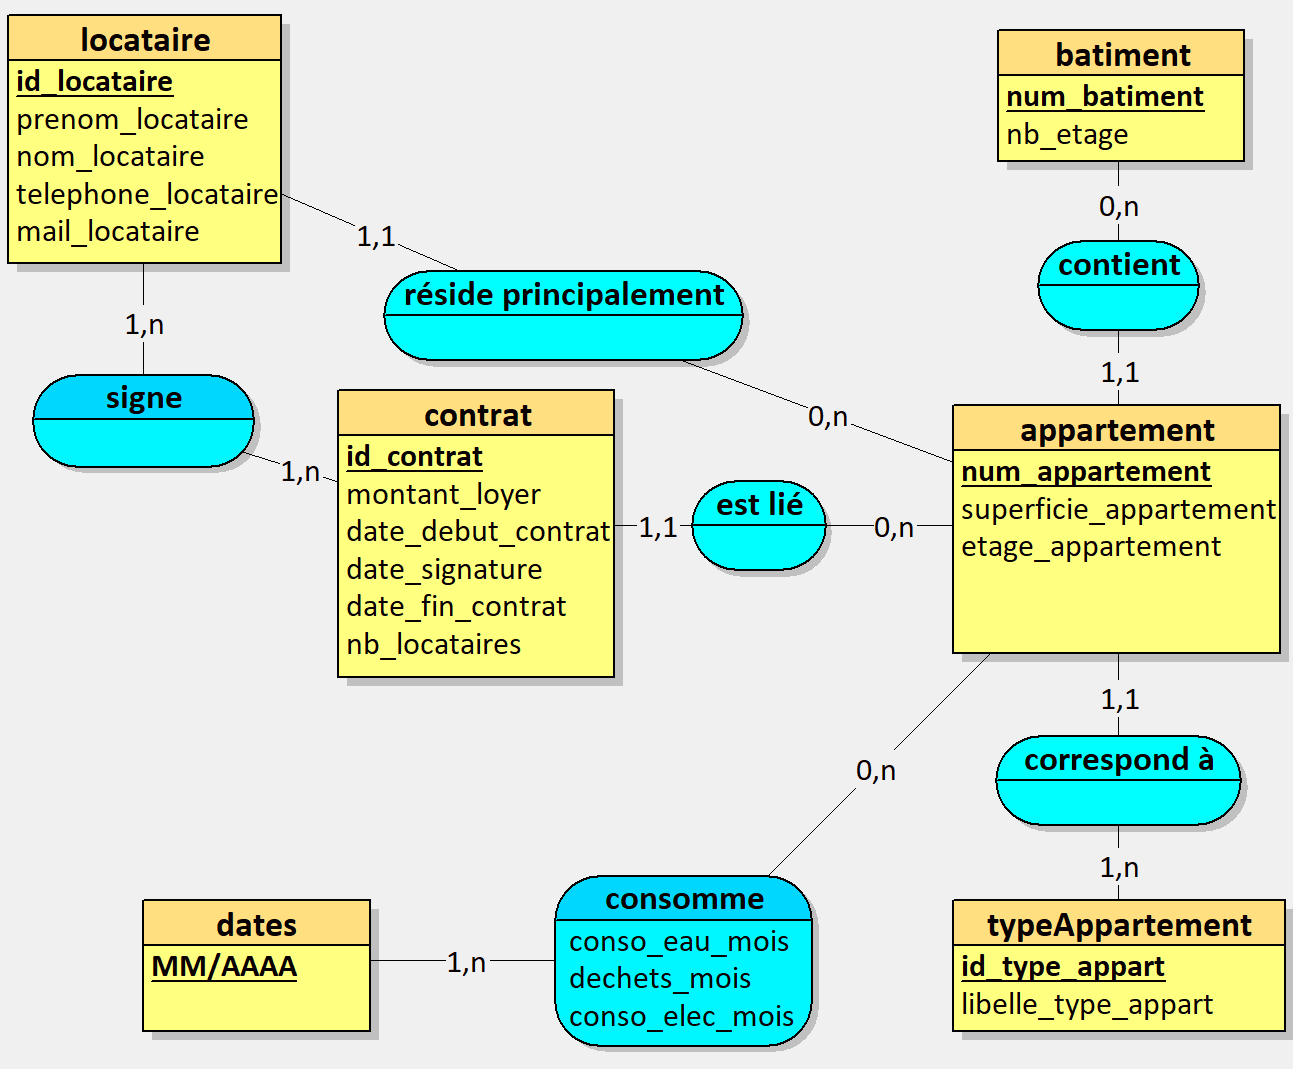
\includegraphics[width=15cm]{mcd.png}
\end{center}
\caption{Modèle conceptuel de données permettant de répondre au besoin énoncé plus tôt}
\end{figure}

\section{Explication et Justification de ce choix}

\subsection{Locataires et Contrats}

Nous avons créé l’entité locataire, qui sera identifiable par id\_locataire, cette entité contiendra le prénom, le nom, le téléphone et le mail de chaque locataire afin d’avoir leur contact complet. Un contrat est associé à un locataire par une signature, ce même contrat sera identifiable par l’identifiant id\_contrat, et contiendra le prix du loyer, la date de début du contrat, la date de signature, la date de fin du contrat et le nombre de locataires. Ces informations permettront de calculer la durée d’un contrat mais aussi de comprendre qu'une consommation puisse être plus élevé dans un appartement habité par plusieurs personnes. Par ailleurs, nous avons choisi comme cardinalité 1,n des deux côtés de l'association "signe" car un contrat doit être signé par minimum un locataire mais peut-être signé par plusieurs locataires dans le cas d'une colocation. De la même façon un contrat peut contenir 1 ou plusieurs locataire (mais jamais aucun sinon ce contrat n'a pas d'intérêt).

\subsection{Bâtiments et Appartements}

Un contrat permet à un locataire de louer un seul appartement comme l'indique la cardinalité 1,1 sortant de contrat vers appartement, en revanche, on conservera tous les contrats qui ont été liés à un appartement comme l'indique la cardinalité 0,n à droite de l'association "est lié" (on considère aussi qu’il est possible qu’un appartement qui vient d’être ajouté dans la base de données puisse ne pas avoir de contrat). L’entité appartement contient son numéro (unique pour chaque appartement permettant d'être l'identifiant de cette entité), la superficie de celui-ci, et le numéro d’étage. On notera aussi qu'un locataire peut résider principalement dans un seul et unique appartement bien qu'il puisse potentiellement avoir signé plusieurs contrat d'où la cardinalité 1,1 à gauche de l'association et 0,n à droite.\\

L’entité bâtiment sera identifiable par le numéro du bâtiment, cette entité aura une propriété nombre d’étages pour connaître le nombre d’étages du bâtiment. Il y aura une association contient entre l’entité bâtiment et l’entité appartement. En effet, l’entité bâtiment peut ne pas avoir d’appartements ou en contenir plusieurs, d’où la cardinalité de 0,n. Cependant, un appartement doit obligatoirement appartenir à un bâtiment et ne peut appartenir qu’à un seul bâtiment, nous avons donc comme cardinalité 1,1.
	 
Nous avons également une entité type d’appartement nous permettant de connaitre le nombre de pièces des appartements. Un appartement ne peut correspondre qu'a un seul type (cardinalité 1,1 vers typeAppartement) mais plusieurs appartement peuvent avoir le même type (cardinalité 1,n de typeAppartement vers appartement). On considère qu'un type n'existe pas tant qu'il n'a pas été employé pour concevoir un appartement.

\subsection{consommation}

L'association consomme entre l’entité appartement et l’entité dates porte les propriétés de consommation d'eau, d'électricité et les déchets produits. On pourra conserver un historique grâce à l'entité dates. Un appartement peut ne pas avoir de consommation d’eau, d’électricité et de déchets ou peut un ou plusieurs relevé de sa consommations qui lui sont reliés d'où une cardinalité de 0,n d'appartement vers l'association consomme.\\

Une date ne sera enregistré que si une consommation a été relevé durant cette dernière. Il va de soit qu'à une date peut correspondre plusieurs relevés provenant de différents appartements d'où le choix d'une cardinalité 1,n de consomme vers dates.
